\section{Geometric Interpretation}\label{sec:geom}
In this section, we present a geometric interpretation of the algorithm based on the Kaczmarz method \cite{kaczmarz1937}. In Section \ref{section:kaczmar-method}, we explain the Kaczmarz method \cite{kaczmarz1937} to solve linear systems. Then in Section \ref{section:geometric-view}, we provide a geometric interpretation of \texttt{SimpleSolver} algorithm based on the Kaczmarz method \cite{kaczmarz1937}. In particular, the \texttt{SimpleSolver} algorithm can be recast as an instance of the randomized Kaczmarz method of Strohmer and Vershynin \cite{Strohmer2007}.

\subsection{Kaczmarz Method}
\label{section:kaczmar-method}
The original Kaczmarz algorithm is an iterative algorithm that solves the linear system $Ax = b$, where $\mathbf{A} \in \mathds{R}^{n \times d}$, $x \in \mathds{R}^d$, $b \in \mathds{R}^n$. If we find out a vector $x$ which satisfies $\mathbf{A}x=b$, this vector will simultaneously satisfy all the following constraints.
\begin{equation}
    \begin{cases}
            a_1 x =b_1 \\
            a_2 x =b_2 \\
            \vdots \\
            a_n x =b_n \\
    \end{cases}
\end{equation}
where $a_i$ is the $i$-th row of matrix $\mathbf{A}$. Each constraint can be shown with a hyperplane in $\mathds{R}^d$ space and the solution for the linear system should be in the intersection of these hyperplanes.
\begin{equation}
    \label{eq:hyperplanes}
    \begin{cases}
        H_1 = \{x : a_1 x=b_1\} \\
        H_2 = \{x : a_2 x=b_2\} \\
        \vdots \\
        H_n = \{x : a_n x=b_n\}
    \end{cases}
\end{equation}
In the Kaczmarz method, we initialize from a random point in $\mathds{R}^d$ space, and in each iteration, we project the point on one of the hyperplanes. Algorithm \ref{alg:Kaczmarz} summarizes the Kaczmarz method.

\begin{algorithm} 
\caption{Kaczmarz Algorithm for linear system $\mathbf{A}x=b$}\label{alg:Kaczmarz}
\begin{algorithmic}[1]
\Require $x_{0}$   
\While{$k \leq C$}            
        \State	$x_{k+1}=x_{k}+\frac{b_{i(k)}-<a_{i(k)},x_{k}>}{\| a_{i(k)}\|^2}a_{i(k)}$
        \State	$i(k)=(k $~ mod ~$n)+1$
        \State	$k=k+1$
\EndWhile
\end{algorithmic}
\textbf{Return} $x_{C+1}$
\end{algorithm}
Figure \ref{fig:kaczmarz} shows eight iteration of Kaczmarz algorithm with $\mathbf{A} \in \mathds{R}^{4 \times 2}$. Therefore, we will have four hyperplanes in two dimensional space. As can be seen in Figure \ref{fig:kaczmarz}, we start from a random point $x_0$, project it on the first hyperplane $H_1$, and obtain $x_1$. In the second iteration, we project $x_0$ to the second hyperplane $H_2$ and achieve $x_2$. We continue this method until we find out the optimal solution $x^*$ or we become very close to the optimal solution.
\begin{figure}[!h]
    \centering
    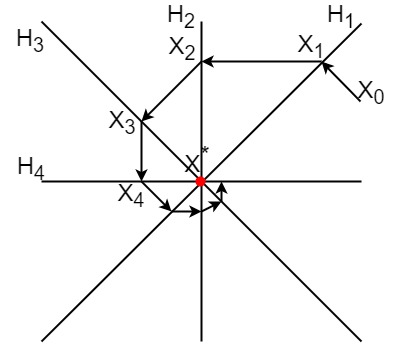
\includegraphics[scale=0.4]{Images/GeometricInterpretation/kacmarz_algorithm.jpg}
    \caption{An example of Kaczmarz method for $\mathbf{A} \in \mathds{R}^{4 \times 2}$}
    \label{fig:kaczmarz}
\end{figure}\\
From a mathematical perspective, it can be shown that the Kaczmarz algorithm can approach the optimal solution very fast. Equation \ref{eq:kaczmarz-convergence} states that in each iteration we approach the optimal solution $x^*$ more than $\|x_{t+1}-x_t\|$.
\begin{equation}
\label{eq:kaczmarz-convergence}
    \forall x^* \in \cap_{i=1}^n H_i,~~~~~~\|x_{t+1}-x^*\|^2 \leq \|x_{t}-x^*\|^2 - \|x_{t+1}-x_t\|^2
\end{equation}

\subsection{Geometric View}
\label{section:geometric-view}
Given the low-stretch spanning tree $T$, we define the cycle basis of $G$ as $\{\overrightarrow{c}_e\}_{e \in E \setminus T}$. The cycle basis includes independent cycles, which correspond to each edge of the graph outside of the spanning tree. In other words, each cycle has just one edge outside of the tree and other edges are on the spanning tree. 

% Figure \ref{fig:cycle} shows an example of a graph with 4 cycle basis $c_1$ to $c_4$. In Figure \ref{fig:cycle}, the low-stretch spanning tree is shown with red edges. Cycle basis $c_1$, $c_2$, $c_3$, and $c_4$ correspond to blue, brown, purple, and green edges in the graph.
% \begin{figure}[!h]
%     \centering
%     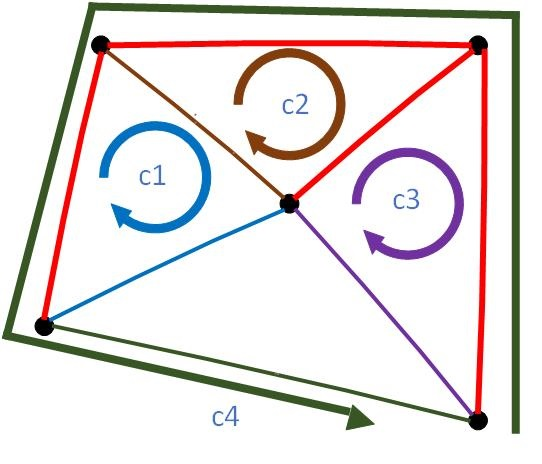
\includegraphics[scale=0.4]{Images/GeometricInterpretation/cycles.jpg}
%     \caption{An example of cycle basis in the graph }
%     \label{fig:cycle}
% \end{figure}\\

Using the cycle basis $\{\overrightarrow{c}_e\}_{e \in E \setminus T}$, we can define the hyperplanes $P_e \stackrel{\text{def}}{=} \{\overrightarrow{f} \in \mathds{R}^E: \overrightarrow{f}^\top R \overrightarrow{c_e}=0\}$ that respect the KPL condition over circulation $\overrightarrow{c}_e$. Then, the optimality condition with respect to a basis of the cycle space can be viewed as requiring the flow $\overrightarrow{f}$ to be in the intersection of the $(m-n+1)$ hyperplanes $\{P_e\}_{e \in E \setminus T}$.
From this geometric perspective, at every iteration, the \texttt{SimpleSolver} algorithm picks a hyperplane $P_e$ associated with
a basis vector $\overrightarrow{c}_e$, and projects the current flow $\overrightarrow{f}_i$ onto $P_e$ as follows.
\begin{equation}
\label{eq:geometric-projection}
    \Pi_{e_i} \overrightarrow{f_i}=(I-\frac{\overrightarrow{c_{e_i}}\overrightarrow{c_{e_i}}^\top R}{\|\overrightarrow{c_{e_i}}\|_R^2})\overrightarrow{f_i}=\overrightarrow{f_i} - \frac{\overrightarrow{f_i}^\top R \overrightarrow{c_{e_i}}}{\|\overrightarrow{c_{e_i}}\|_R^2}\overrightarrow{c_{e_i}}=\overrightarrow{f_{i+1}}
\end{equation}
Notice that, as this update adds a circulation to $\overrightarrow{f}_i$, the resulting flow $\overrightarrow{f}_{i+1}$ meets the demands $\overrightarrow{\chi}$. 

% Furthermore, it is worth mentioning that in the \texttt{SimpleSolver} algorithm the inner product is a bit different from the classical inner product. We define $<\overrightarrow{f}_i, \overrightarrow{c}_{e_i}>_{\mathbf{R}}=\overrightarrow{f}_i^\top \mathbf{R} \overrightarrow{c}_{e_i}$ and $\| \overrightarrow{c}_{e_i} \|_{\mathbf{R}}^2=\\
% <\overrightarrow{c}_{e_i}, \overrightarrow{c}_{e_i}>_{\mathbf{R}}=\overrightarrow{c}_{e_i}^\top \mathbf{R} \overrightarrow{c}_{e_i}$. Therefore, in \texttt{SimpleSolver} algorithm, $\overrightarrow{f}_{i}$ and $\overrightarrow{c}_{e_i}$ correspond to $x_k$ and $a_{i(k)}$ in Kaczmarz algorithm, respectively. $b_{i(k)}$ is zero in \texttt{SimpleSolver} algorithm. If we change the inner product and norm in the Kaczmarz algorithm to the $<.,.>_{\mathbf{R}}$ and $\|.\|_{\mathbf{R}}$, we can easily obtain Equation \ref{eq:geometric-projection} for \texttt{SimpleSolver} algorithm.
% \begin{center}
%     $x_{k+1}=x_{k}+\frac{b_{i(k)}-<a_{i(k)},x_{k}>}{\| a_{i(k)}\|^2}a_{i(k)}=x_{k}+\frac{b_{i(k)}-<x_{k},a_{i(k)}>}{\| a_{i(k)}\|^2}a_{i(k)}$
% \end{center}
% \begin{equation}
%     \overrightarrow{f}_{i+1}=\overrightarrow{f}_i+\frac{0-<\overrightarrow{f}_i,\overrightarrow{c}_{e_i}>_{\mathbf{R}}}{\| \overrightarrow{c}_{e_i} \|_{\mathbf{R}}^2} \overrightarrow{c}_{e_i}=\overrightarrow{f}_i-\frac{\overrightarrow{f}_i^\top \mathbf{R} \overrightarrow{c}_{e_i}}{\| \overrightarrow{c}_{e_i} \|_{\mathbf{R}}^2}\overrightarrow{c}_{e_i}
% \end{equation}

% New version of previous para by Danya
Generally speaking, given an inner product $\langle ., . \rangle$, the orthogonal projection of $x$ along $y$ (resp. $y^\perp$) in that inner product space is $Proj_y(x) = \frac{\langle y, x \rangle }{ \langle y , y\rangle}y$ (resp. $Proj_{y^\perp}(x) = x - \frac{\langle y, x \rangle}{ \langle y , y\rangle}y$). Noting that $\langle \overrightarrow a , \overrightarrow b \rangle = \overrightarrow a^T R\overrightarrow b$ is an inner product, denote $S$ the inner product space with this inner product. Since $\| \overrightarrow a \|^2_R = \langle \overrightarrow a, \overrightarrow a \rangle$, we can see that the above expression $\overrightarrow f_i - \frac{\overrightarrow f_i^T R \overrightarrow c_{e_i}  }{\| \overrightarrow c_{e_i}\|^2_R} c_{e_i}$ is an orthogonal projection of $\overrightarrow f_i$ along $\overrightarrow c_{e_i}^\perp$ in $S$, in the ordinary sense of projection, meaning that this projection operator $\Pi_{e_i}$ is symmetric and idempotent. 